\section{Motivation}

\begin{frame}{Why Lighting Matters}
  \vspace{0.5cm}
  \pause
  \begin{minipage}{0.45\textwidth}
    \centering
    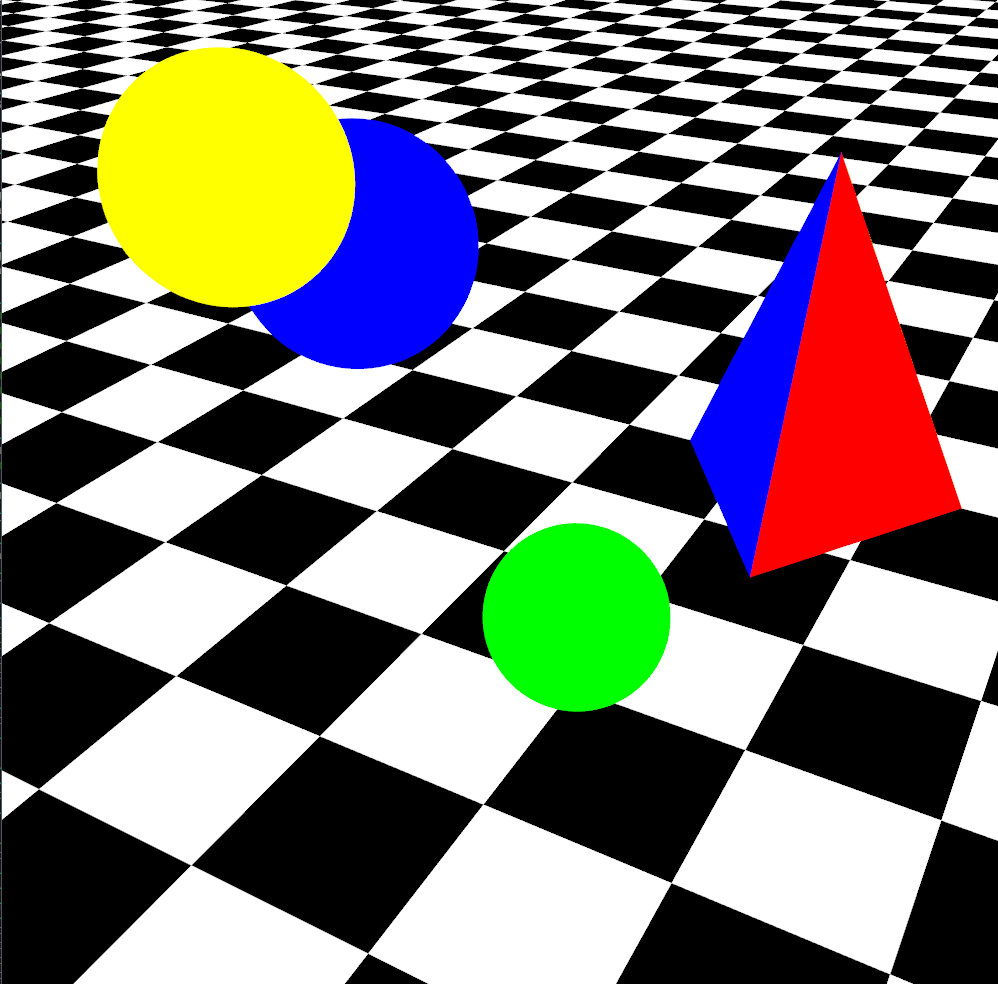
\includegraphics[width=\linewidth]{images/flat.png}
    \captionof*{figure}{Without Lighting and Shading}
  \end{minipage}%
  \hfill
  \pause
  \begin{minipage}{0.45\textwidth}
    \centering
    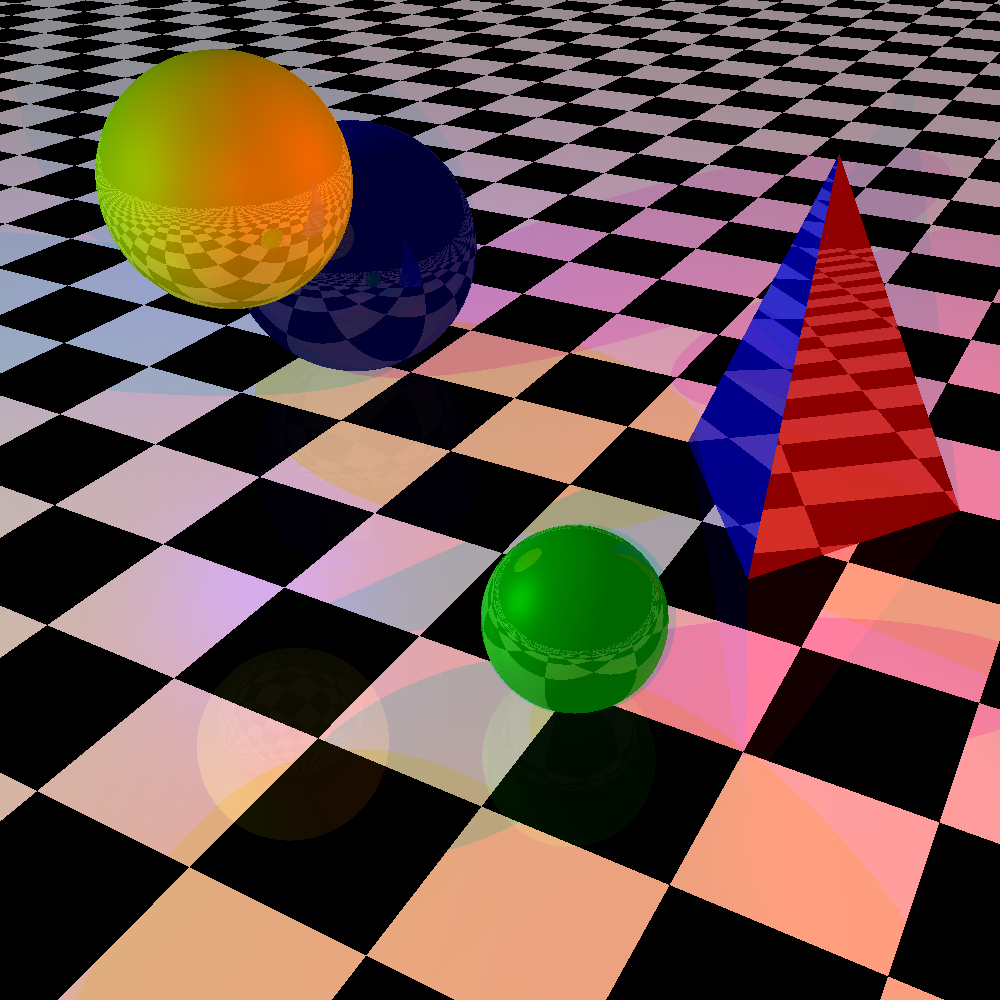
\includegraphics[width=\linewidth]{images/rtx.png}
    \captionof*{figure}{With Lighting and Shading}
  \end{minipage}

  \begin{itemize}
    \item<3-> \textbf{Depth perception} - Lighting reveals 3D shape and form
    \item<4-> \textbf{Material properties} - Distinguishes between plastic, metal, wood
    \item<5-> \textbf{Realism} - Makes computer graphics believable and immersive
  \end{itemize}
\end{frame}

\begin{frame}{The Challenge: From Reality to Code}
  \begin{columns}
    \begin{column}{0.5\textwidth}
      \begin{tikzpicture}[scale=0.8]

        \begin{scope}[plane x={(0.866,0.5,0)}, plane y={(0, 0.5, -0.866)}, canvas is plane]
          \draw[ObjectColor, fill=ObjectColor!20] (1.5,-2) rectangle (5, 1);
          \node[below] at (3,-2.5) {\small \objectcolor{Surface}};
        \end{scope}

        \node[circle, fill=LightColor, minimum size=1cm] (sun) at (0,3) {\faIcon{sun}};
        \node[below] at (0,4.25) {\small \textcolor{LightColor}{Light Source}};

        \draw[lightray] (sun) -- (2,1.5);
        \draw[lightray] (sun) -- (2.5,1);
        \draw[lightray] (sun) -- (3,1.5);
        \draw[lightray] (sun) -- (3.5,1);

        \draw[reflectray] (2,1.5) -- (1,3);
        \draw[reflectray] (2.5,1) -- (1.5,3);
        \draw[reflectray] (3,1.5) -- (2,3);
        \draw[reflectray] (3.5,1) -- (2.5,3);

        \node[eye] (eye) at (5,2) {\faIcon{eye}};
        \node[below] at (5,1.5) {\small Observer};
      \end{tikzpicture}
    \end{column}
    \pause
    \begin{column}{0.5\textwidth}
      \begin{conceptbox}{Reality vs Computation}
        \textbf{Physical World:}
        \begin{itemize}
            \footnotesize
          \item Millions of photons per surface point
          \item Complex wave interactions
          \item Multiple scattering events
          \item Continuous spectrum
        \end{itemize}

        \vspace{0.3cm}
        \textbf{Computer Graphics:}
        \begin{itemize}
            \footnotesize
          \item Discrete RGB values
          \item Simplified mathematical models
          \item Local illumination approximations
          \item Real-time constraints
        \end{itemize}
      \end{conceptbox}
    \end{column}
  \end{columns}
\end{frame}
